\label{chapter:hmr_sim}

Conforme comentado no Capítulo \ref{chap:introduction}, a proposta deste projeto é fornecer uma ferramenta direcionada para simulação de sistemas multi-robôs auto-adaptativo com baixo nível de detalhamento físico. Essa porposta foi realizada através do simulador HMR Sim. É um projeto \textit{open source}, disponível em \url{https://github.com/lesunb/HMRSsim}.

A linguagem escolhida foi Python, uma linguagem de programação popular e versátil. Outros simuladores analisados têm suporte para essa linguagem, como MORSE e CoppeliaSim. Arquitetura do simulador é baseado na \textit{design pattern} Entity-Component-System (ECS), e a técnica de simulação é de eventos discretos. Grande foco foi dado para modularização e reaproveitamento de sistemas na construção do simulador. Alguns dos principais sistemas (e.g. Navegação, Script) foram construídos para serem extensíveis. Além disso foi dado atenção à facilidade e rapidez de construir simulações. A arquitetura do simulador é detalhada na Seção \ref{sec:architecture}. A criação e uso de sistemas na Seção \ref{sec:systems}. Os principais sistemas já construídos são apresentados na Seção \ref{sec:systems_available}, incluindo o sistema que permite visualização da simulação, Seer. Finalmente a Seção \ref{sec:performance} verifica o desempenho do simulador numa simulação com grande número de robôs.

Uma simulação no HMR Sim tem dois estágios: (1) fase de carregamento, onde os componentes disponíveis são carregados e as entidades da simulação criadas e (2) fase de execução, onde os sistemas da simulação são inicializados e a simulação em si é executada. Componentes são definidos como classes em Python e são carregados automaticamete utilizando um sistema de nomenclatura apropriado. Sistemas são construídos como funções Python, e podem ser processos da biblioteca \texttt{simpy} ou funções aceitas como sistemas do \texttt{esper} (ver Seções \ref{sec:simulation_techniques} e \ref{sec:ECS} para detalhes sobre as bibliotecas). Os sistemas devem ser inicializados e adicionados ao simulador antes da fase de execução. A Seção \ref{sec:ents_and_components} cobre a criação de componentes e como eles ficam disponíveis no simulador.

Uma simulação pode ser definida em um mapa (veja figura \ref{fig:example_map}), programaticamente através de um objeto de configuração (dicionário Python), ou uma mistura das duas opções. Mapas são arquivos XML construídos com a biblioteca \texttt{JGraph} (disponível em \url{https://github.com/jgraph}), com algumas restrições. Qualquer programa compatível com essa biblioteca pode ser utilizado, por exemplo \url{diagrams.net}, bastante popular. Também é possível criar entidades na simulação através de \textit{EntityDefinition}.

As formas desenhadas no mapa da simulação podem ser anotadas para especializá-las (marcar a figura como um certo tipo de entidade), adicionar componentes, ou diferenciá-la de alguma forma. Na figura \ref{fig:example_annotations}, por exemplo, as anotações marcam aquele objeto do mapa como um robo, que possui um componente \texttt{Claw} inicializado com os valores \texttt{[80, 1]}, e um componente \texttt{Script} inicializado com os valores da figura.

\begin{figure}[ht]
    \centering
    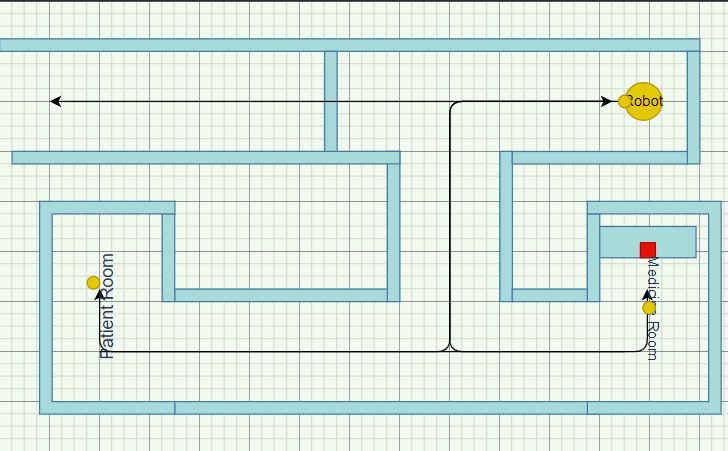
\includegraphics[width=.8\textwidth]{map_example.png}
    \caption{Exemplo de mapa de uma simulação}
    \label{fig:example_map}
\end{figure}

\begin{figure}[ht]
    \centering
    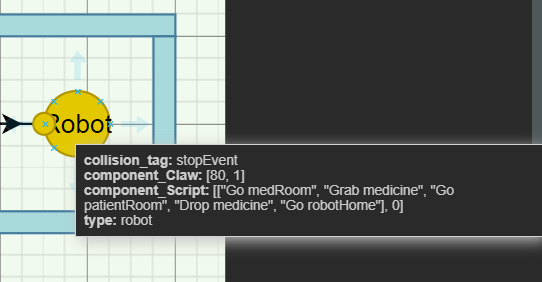
\includegraphics[width=.8\textwidth]{robot_annotations.png}
    \caption{Exemplo de anotações em uma entidade}
    \label{fig:example_annotations}
\end{figure}


\section{Arquitetura}
\label{sec:architecture}

\begin{figure}[ht]
    \centering
    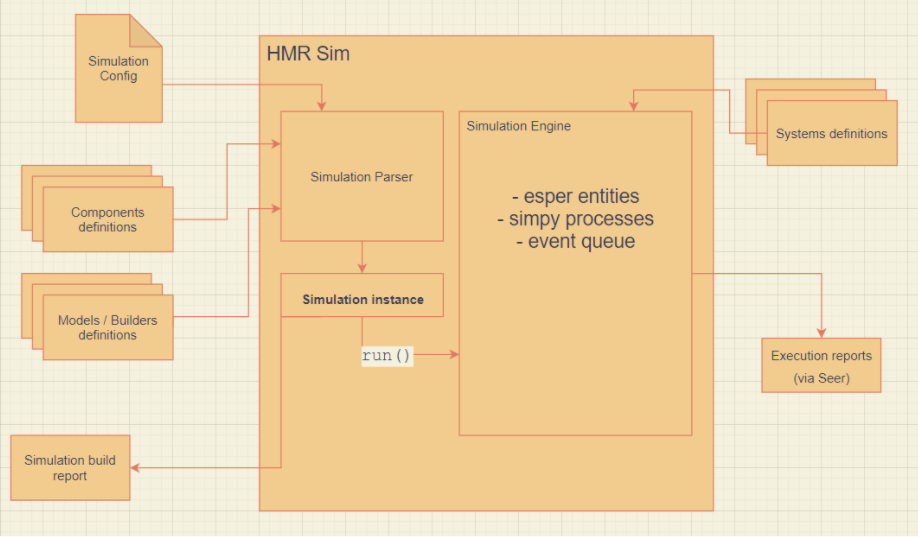
\includegraphics[width=\textwidth]{architecture_overview.png}
    \caption{Diagrama representando um resumo da arquitetura do HMR Sim}
    \label{fig:architecture_overview}
    \gab{reexportar imagem como pdf}
\end{figure}

A figura \ref{fig:architecture_overview} mostra um resumo da arquitetura do simulador HMR Sim. A construção da simulação acontece separada da simulação em si. Para construir uma simulação, um objeto de configuração tem que ser passado para o simulador, bem como as definições dos componentes disponíveis e os \texttt{models} e \texttt{builders} disponíveis. A classe \texttt{Simulator} cria a simulação, e depois a executa. A instancia da simulação mostrada na figura \ref{fig:architecture_overview} (\textit{Simulation instance}) é exatamente a instância da classe \texttt{Simulator} criada.

O objeto de configuração é um dicionário Python, que pode ser salvo como um arquivo \texttt{json}. Algumas das opções mais importantes estão listadas abaixo. Para ver todas as opções verifique a documentação do projeto, no repositório.

\begin{itemize}
    \item \textbf{context} (string) - A raíz do projeto, de onde componentes, sistemas e builders extras serão incluídos;
    \item \textbf{map} (string) - O arquivo XML do mapa
    \item \textbf{FPS} (int) - Frequência com que serão executados os sistemas do \texttt{esper}. Esses sistemas não geram eventos, são indicados para representar sistemas que acontecem de forma frequênte e previsível. Caso nenhum sistema \texttt{esper} seja utilizado não é necessário informar esse valor.
    \item \textbf{duration} (int) - Tempo limite da simulação (no relógio da simulação). Por exemplo, um valor 6 vai fazer o simulador encerrar a simulação após 6s serem simulados.
    \item \textbf{simulationComponents} (dict) - Componentes "globais". Eles são adicionados à entidade 1, reservada à simulação. Podem ser acessados por todos os robôs (e.g. um mapa compartilhado de rotas).
    \item \textbf{extraEntities} (EntityDefinition[]) - Lista de \texttt{EntityDefinition} (ver documentação), que definiem entidades que não estão presentes no mapa mas devem ser incluídas na simulação. É possível declarar todas as entidades com essa opção e usar o mapa apenas para coisas estáticas, reaproveitando-o para vários cenários. 
\end{itemize}

O simulador importa automaticamente \texttt{components}, \texttt{models} e \texttt{builders} do sistema de arquivos. Por conta disso os projetos que usem o HMR Sim precisam de uma organização expecífica, como mostrado abaixo. Dentro de cada pasta os arquivos deve estar no formato apropriado.

\begin{lstlisting}[]
                   project_root     
                    |                 
                    |-- models        
                    |-- components    
                    |-- builders      
\end{lstlisting}

A simulação construída se torna uma instância da classe \texttt{Simulator} cujo atributo \texttt{World} está preenchido com as entidades que foram criadas, e as opções de configuração salvas. Essa instância é um objeto Python, podendo ser salvo através da biblioteca \texttt{pickle}, por exemplo, e distribuído. Antes de poder ser executada, no entanto, é necessário inicializar e adicionar os sistemas à simulação. Para adicionar sistemas os métodos \texttt{Simulator.add\_system} e \texttt{Simulator.add\_des\_system} podem ser usados. Qual dos dois usar depende do sistema a ser adicionado, detalhes na Seção \ref{sec:systems}.

Após adicionar os sistemas, a simulação pode ser executada utilizando o método \texttt{Simulator.run}, da instância do simulador gerada. A simulação é executada por \texttt{duration} segundos de simulação, se essa opção foi passada na configuração, ou até que o evento \texttt{KILL\_SWITCH} seja processado. É possível manter ver logs da simulação durante a execução. A visualização gráfica da simulação é implementada através do sistema Seer, discutido na seção \ref{sec:seer}.

Alguns sistemas com funcionalidades consideradas essenciais na maior parte das simulações já foram implementados, como parte da validação do simulador. Eles serão detalhados na Seção \ref{sec:systems_available}, e incluem sistema de navegação, movimentação, colisão, controle de robôs, sensores, e visualização.

\section{\texttt{builders} e \texttt{models}}
\label{sec:builders_and_models}

Os arquivos XML que podem ser usados de mapas representam os objetos desenhados dentro de tags \texttt{<mxCell>}, com alguma geometria. Diferentes formas possuem diferentes conteúdos na tag \texttt{<mxCell>}. \texttt{models} são funções que traduzem o XML em uma \texttt{<mxCell>} para uma lista de componentes da simulação. Cada \texttt{model} deve ser armazenado em um arquivo próprio que exporte: (1) uma função \texttt{from\_mxCell}, que recebe uma \texttt{<mxCell>} e retorna uma lista de componentes; (2) uma constante \texttt{MODEL} com o nome da forma que esse model traduz.

\texttt{builders} são semelhantes aos \texttt{models}, mas fazem a tradução do XML contido em \texttt{<object>}. Qualquer forma (\texttt{<mxCell>}) que tenha anotações (como as mostradas na figura \ref{fig:example_annotations}) é envolvida em uma tag \texttt{<object>} que guarda as anotações. \texttt{builders} traduzem tanto as anotações no objeto quanto o XML da \texttt{<mxCell>} contido nele. Eles podem ou não fazer uso de \texttt{models} para isso. UM \texttt{builder} deve estar em um arquivo próprio que exporte: (1) uma função \texttt{build\_object}, que transforma o XML do objeto e (2) uma constante \texttt{TYPE}, indicando que esse \texttt{builder} deve ser aplicado em objetos que tenham a anotação \texttt{type} com esse valor.

Os \texttt{models} e \texttt{builders} são opcionais. Caso todas as entidades sejam criadas através da opção \texttt{extraEntities} da configuração eles serão desnecessários. Atualmente cerca de 10 formas podem ser usadas, e cerca de 7 \texttt{builders} foram criados.

\section{Entidades e Componentes}
\label{sec:ents_and_components}

HMR Sim utiliza a biblioteca \texttt{esper} \cite{esper} (ver detalhes na Seção \ref{sec:ECS}) para gerenciar as entidades e seus componentes na simulação. Cada entidade do mapa ou das entidades passadas pela configuração é representada por um inteiro, armazenado dentro da classe \texttt{World} do \texttt{esper}, e pode ser acessado através da instância da simulação no atributo \texttt{world}, e também pelos sistemas. O identificador de cada objeto do mapa e qual entidade corresponde a ele fica armazenado no atributo \texttt{draw2ent} do simulador. Entidades também podem ser adicionadas diretamente à simulação através do método \texttt{Simulator.add\_entity}.

Entidades possuem um conjunto de componentes. componentes podem ser adicionados ou removidos de entidades usando métodos da biblioteca \texttt{esper}. Existem também métodos para verificar a existência de um componente em uma entidade, buscar componentes específicos de entidades, buscar todos os componentes de um certo tipo no \texttt{World}, etc. Componentes são simplesmente classes Python, que devem ter o mesmo nome que o arquivo que as declara (uma por arquivo). É convencionado no padrão ECS que os componentes não tenham lógica implementada, sugere-se que apenas os métodos \texttt{\_\_init\_\_} e \texttt{\_\_str\_\_} sejam implementados em um componente. \texttt{@dataclass} podem ser utilizadas. 

O identificador de um componente é o nome da sua classe. Dessa forma, se o componente \texttt{simulator.componentes.MyComponent} for declarado, para utilizá-lo em algum sistema pode-se importá-lo normalmente (e.g. \texttt{from simulator.components.MyComponent import MyComponent}) e usar essa importação ao se referir ao componente (buscando-o no \texttt{World}, por exemplo).

\section{Sistemas}
\label{sec:systems}

Sistemas são uma parte essencial do simulador, pois são os responsáveis por fazerem a simulação acontecer. Sistemas são também muito versáteis, podendo ser usados não só para representar uma parte da simulação, mas também para extrair informações dela. Existem 2 tipos diferentes de sistemas que podem ser usados: um sistema compatível com sistemas da biblioteca \texttt{esper}, referidos como "sistemas normais" e sistemas compatíveis com a biblioteca \texttt{simpy}, referidos como "sistemas DES". Ambos são opcionais e o uso de um ou outro depende do que será simulado pelo sistema. As seções \ref{sec:normal_systems} e \ref{sec:des_systems} explicam a diferença entre eles e as particularidades de cada um.

O conceito central do HMR Sim é que sistemas são construídos para utilizar um conjunto de componentes e representar uma parte da simulação. Cada conjunto de sistemas relacionados (e seus componentes) confere novas capacidades ao simulador, e portanto à simulação sendo feita, por exemplo sistemas podem representar sensores, movimentação, comunicação entre robôs, etc. Grande parte da flexibilidade que o simulador proporciona está na relativa facilidade de criar e usar sistemas. Se algum sistema não se adequa às suas necessidades, basta substituí-lo por outro, ou modificá-lo, sem ter que alterar outras partes da simulação. Por exemplo, se o objetivo de uma simulação é comparar dois algoritmos de gerenciamento de robôs, 2 sistemas diferentes (que usem os mesmos componentes) serão criados, um para cada algoritmo. Testar o algoritmo A ou B se torna uma simples questão de adicionar o sistema A ou B na simulação.

\subsection{Sistemas compatíveis com \texttt{esper}}
\label{sec:normal_systems}

Os "sistemas normais" são aqueles que ficam armazenados dentro do \texttt{World} do \texttt{esper}. Eles são definidor como classes que extendem a classe \texttt{esper.Processor} e devem implementar 2 funções: \texttt{\_\_init\_\_} e \texttt{process}. A função \texttt{process} recebe dois argumentos, \texttt{self}, a instância do \texttt{World}  e \texttt{kwargs}, os parâmetros passados pelo \texttt{Simulator} aos sistemas (ver documentação).

Esses sistemas (e apenas eles) são executados pelo \texttt{esper}. Para utilizzá-los é necessário passar a opção \texttt{FPS} na configuração da simulação. Esses sistemas serão então executados uma vez a cada $\frac{1}{FPS}$ segundos de simulação. Note que o uso desses sitemas força a simulação a correr em passos (i.e. o relógio da simulação vai andar em intervalos de, no máximo, $\frac{1}{FPS}$).

Esse tipo de sistema é indicado para simular comportamentos constantes e repetitivos, com frequência definida. Por exemplo movimentação, verificação de colisão, aumento de temperatura em uma sala, gasto de bateria, etc. Eles geralmente seguem o formato mostrado no código \ref{code:normal_system}

\begin{adjustwidth}{-1cm}{0cm}
\lstinputlisting[language=Python, basicstyle=\ttfamily\small, captionpos=b,caption=Formato básico de um sistema normal, label=code:normal_system]{snippets/normal_system_scaffold.py}
\end{adjustwidth}

\subsection{Sistemas compatíveis com \texttt{simpy}}
\label{sec:des_systems}

Os "sistemas DES" são gerenciados pelo \texttt{simpy}. Eles são definidos como processos do \texttt{simpy}, e podem ser qualquer processo aceito pelo \texttt{simpy}, ou seja, qualquer função geradora. Sugere-se, como convenção, usar uma função chamada \texttt{process}. Opcionalmente podem também definir uma função de limpeza, que será executada ao final da simulação, e serve para fechar arquivos que foram abertos, por exemplo. Esses sistemas "vivem" todos dentro do mesmo ambiente do \texttt{simpy}, que é armazenado como um dos atributos da simulação.

A comunicação entre esse tipo de sistema aproveita os eventos suportados pelo \texttt{simpy}, utilizando o recurso \texttt{EVENT\_STORE}, outro atributo do simulador. Convenciona-se que apenas eventos (\texttt{EVENT} ou \texttt{ERROR}, ver \texttt{typehints} na documentação do simulador) sejam utilizados dentro da \texttt{EVENT\_STORE}. Cada sistem pode exportar seu próprio payload e tag para eventos. Assim, qualquer outro sistema que queira enviar uma mensagem para o sistema em questão só precisa criar um novo evento com o payload e tag apropriado e adicioná-lo a \texttt{EVENT\_STORE}. Esse sistema de comunicação permite a criação de sistemas reativos, que apenas processam eventos esperados por eles, e no resto do tempo ficam desativados.

É possível também um sistema em determinado momento criar um canal temporário para aguardar uma resposta de alguma operação asíncrona. É possível também que um sistema execute em mais de uma thread, mas a thread principal deve executar na mesma que o resto do simulador, e deve ser adicionada ao ambiente \texttt{simpy}. A comunicação entre as threads so sistema é de responsabilidade dele.

Durante a execução argumento \texttt{kwargs} é passado aos sistemas, dando acesso ao \texttt{World}, ao ambiente \texttt{simpy} da simulação, à \texttt{EVENT\_STORE}, o evento \texttt{KILL\_SWITCH}, etc. Essas informações permitem ao sistema grande poder sobre a simulação. O evento \texttt{KILL\_SWITCH} é um evento especial que termina a simulação se for disparado.

Esses tipo de sistema é indicado para simular comportamentos inconstantes ou imprevisíveis, sistemas reativos ou ainda como plugins, exetendendo o simulador. O código \ref{code:des_system} representa o formato típico de um sistema DES.

\begin{adjustwidth}{-1cm}{0cm}
    \lstinputlisting[language=Python, basicstyle=\ttfamily\small, captionpos=b,caption=Formato básico de um sistema DES, label=code:des_system]{snippets/des_system_scaffold.py}
\end{adjustwidth}
% TODO verificar config hightlight python

\section{Sistemas Disponíveis}
\label{sec:systems_available}

Alguns sistemas considerados críticos foram implementados no desenvolvimento desse projeto. Eles serviram parcialmente como validação das decisões tomadas ao longo do projeto. Ao longo do seu desenvolvimento foi dado foto na modularização e extensibilidade, como evidenciado principalmente nos sistemas de controle de entidades e navegação. Todos os sistemas que serão citados nas próximas seções (Seções \ref{sec:movement} até \ref{sec:seer}) foram testados com simulações que estão disponíveis nos exemplos do projeto (\url{https://github.com/lesunb/HMRSsim}).

\subsection{Sistema de Movimentação e Colisão}
\label{sec:movement}

O sistema de movimentação é intimamente relacionado ao sistema de colisão. Ambos foram modelados como sistemas compatíveis à biblioteca \texttt{esper}. Os componentes que habilitam esses sistemas são posição, velocidade e uma caixa de colisão (\texttt{Collidable}). Esses sistemas dão suporte para simulações 2D apenas, para uma simulação 3D outros sistemas precisam ser implementados.

Convenciona-se que apenas o sistema de movimentação modifica o componente posição das entidades. Outros sistemas que queiram movimentar uma entidade devem adicionar velocidade à ela, através do componente de velocidade. Isso permite que o sistema de movimentação seja leve, levando em média 0.003s para movimentar 200 entidades na simulação do enxame de drones (detalhes na Seção \ref{sec:performance}). O sistema de movimentação também é responsáver por dividir o espaço da simulação em setores, para aumentar a eficiência do sistema de colisão. O tamanho do setor pode ser alterado na inicialização do sistema de movimentação.

O sistema de colisão verifica colisão entre entidades que se mexem (i.e. possuem os componentes \texttt{Position}, \texttt{Collidable} e \texttt{Velocity}) e outras entidades da simulação que tenham uma posição e o componente \texttt{Collidable}. Por questões de desempenho apenas formas côncavas são utiliadas, porém é possível definir múltiplas formas para a mesma entidade, aproximando assim um formato convexo. Como mencionado anteriormente, é feita uma separação da simulação em setores, assim o sistema de colisão só verifica colisão de uma entidade com as entidades no mesmo setor e em setores adjacentes na simulação, aumentando a eficiência do sistema em simulações com muitas entidades. Na simulação do enxame de drones, esse sistema apresentou uma média de 0.097s à 0.085s para verificar a colisão das 200 entidades. A diferença ocorre porque em diferentes momentos da simulação as entidades estão mais próximas ou mais separadas, evidenciado que a separação da simulação em setores afeta diretamente o desempenho desse sistema.

Quando uma colisão é detectada, um evento de colisão é adicionado à fila de eventos (i.e. \texttt{EVENT\_STORE}), com os IDs das entidades que colidiram. Um outro sistema deve ser implementado para tomar a resposta apropriada em relação a esse evento, preferencialmente um sistema DES reativo. \texttt{simulator/systems/StopCollisionDESProcessor} é um exemplo de sistema que pode ser utilizado.

\subsection{Sistema de Navegação}
\label{sec:navigation}

O sistema de navegação foi construído para permitir que robôs encontrem caminhos até pontos do mapa por conta própria. Esse sistema funciona em conjunto com o sistema de caminhos, que é baseado em caminhos que o robõ deve seguir (componente \texttt{Path}). Existem duas maneiras de comandar um robô até um ponto específico do mapa: passando uma coordenada do mapa, ou definindo um ponto de interesse (POI) no mapa (ver figura \ref{fig:navigation_map}, os pontos vermelhos), e passando a tag identificadora desse POI para o robô. Esse comando é feito através de eventos na fila de eventos.

É esperado ainda que a entidade do ambiente (entidade 1) tenha um componente \texttt{Map}, o mapa de caminhos que será compartilhado por todos os robôs, e que caminhos tenham sido definidos no mapa, utilizando entidades do tipo \texttt{map-path} (ver figura \ref{fig:navigation_map}, as setas). Esses caminhos são considerados percursos seguros que os robôs podem seguir para se movimentar ao longo do mapa. Durante a criação da simulação, os \texttt{map-paths} são transformados em um grafo armazenado no componente \texttt{Map} do ambiente. Pontos próximo são combinados em "super-pontos" para diminuir a quantidade de nós no grafo, aumentando a eficiência das buscas. O tamanho de um super-ponto pode ser definido na inicialização do componente \texttt{Map}.

\begin{figure}[ht]
    \centering
    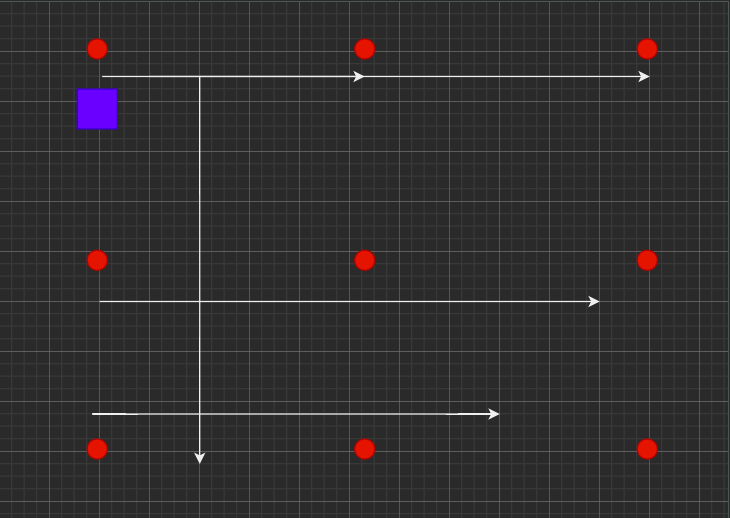
\includegraphics[width=.8\textwidth]{map_poi_test.png}
    \caption{Mapa representando POIs (pontos vermelhos) e \texttt{map-paths} (setas) para o sistema de navegação}
    \label{fig:navigation_map}
\end{figure}

Ao inicializar o sistema de navegação, uma função de navegação deve ser informada. Essa função recebe como parâmetros o mapa do ambiente, a posição atual do robô e sua posição de destino, e deve retornar um caminho (\texttt{Path}) da origem até o destino através dos caminhos seguros do mapa. É permitido que os robôs saiam dos caminhos seguros dentro de um limite que pode ser configurado no componente \texttt{Map}. A função \texttt{find\_route} (\texttt{simulator/systemas/NavigationSystem}) pode ser usada como função que encontra caminhos.

% TODO: Adicionar referência ao projeto do gazebo que usa esse sistema de caminhos
Encontrado um caminho do ponto de origem ao ponto de destino, o componente \texttt{Path} que representa esse caminho a ser seguido é adicionado à entidade. A partir desse ponto o sistema de caminhos (\texttt{PathProcessor}) se encarrega de adicionar velocidade ao robô para que passe por todos os pontos do caminho. Ao chegar no destino, o componente é removido. Caso um caminho não seja encontrado, um evento de erro é adicionado à fila de eventos, para que o controlador do robô (que passou o comando de movimentação) possa tomar a decisão apropriada.

A simulação \texttt{poi\_test} (ver figura \ref{fig:navigation_map}) foi feita para testar o sistema de navegação. Nessa simulação um robô (o quadrado) recebe instruções para ir a alguns POIs (os círculos) em sequência, utilizando o sistema de navegação. Ele segue os caminhos definidos no mapa (as setas). 

Toda vez que uma entidade encontra um caminho até um objetivo, esse caminho encontrado (que pode passar por pontos ainda não mapeados) é incluído ao mapa compartilhado, na tentativa de expandi-lo. Assim, quanto mais as entidades navegam pelo mapa, mais pontos conhecem e mais pontos podem acessar.

\subsection{Sistema de Controle}
\label{sec:scripting}

O sistema de controle (ou sistema de script) foi criado para facilitar o controle e passagem de instruções às entidades da simulação. Ele é especialmente indicado para criar o equivalente a NPCs (\textit{non playable characters}) numa simulação, ou seja, entidades que precisam se movimentar de alguma forma, mas não são o foco da simulação. Esse sistema foi feito para ser extensível por outros sistemas, e funciona baseado em instruções. Na figura \ref{fig:example_annotations}, um dos componentes do robô é \texttt{component\_Script}, que é o componente utilizado pelo sistema de controle. O vetor de strings passados para esse componente é a sequência de instruções que ele vai realizar na simulação, gerenciadas pelo sistema de controle. Esse sistema é reativo e reage à eventos anotados como funções ou como eventos de interesse.

Uma instrução pode ser definida por qualquer sistema, e incluída no sistema de script durante sua inicialização. Elas são implementadas através de funções que aceitem argumentos específicos (detalhes na documentação do projeto), e cujo retorno é o estado do script daquela entidade ao executar a instrução. Por exemplo, na figura \ref{fig:example_annotations} a função \texttt{Go} foi definida pelo sistema de navegação, e as funções \texttt{Grab} e \texttt{Drop} pelo sistema da garra (um atuador que será discutido na Seção \ref{sec:robot_skills}).

Existem 3 estados que um script pode estar ao longo da simulação: \texttt{READY}, \texttt{BLOCKED} ou \texttt{DONE}. \texttt{DONE} significa que todas as instruções do script foram executadas. \texttt{READY} indica que a entidade está pronta para executar a próxima instrução. \texttt{BLOCKED} sinaliza que a entidade está executando alguma ação do script, ou esperando que algo aconteça para poder executar a próxima instrução. Para dar suporte às ações asíncronas, existe uma lista de eventos que o script espera. Toda vez que uma instrução asíncrona é executada, espera-se que o retorno seja o estado \texttt{BLOCKED}, e que tenham sido adicionadas ao componente de script as tags dos eventos que marcam o final da ação sendo executada. O sistema de controle é ativado ao receber um evento com alguma dessas tags, e vai removendo elas da lista de espera do script da entidade apropriada. Quando essa lista fica vazia a entidade é desbloquada (i.e. passa do estado \texttt{BLOCKED} para o estado \texttt{READY}).

Por exemplo, se a entidade $2$ vai executar a instrução \texttt{Go poi}. Essa instrução pode emitir um evento para o sistema de navegação movimentar a entidade $2$ até a coordenada do ponto de interesse "poi". Quando o robô chegar até o ponto de destino, nesse sistema, é emitido um evento \texttt{EndOfPath}. Nesse caso, a função que implementa a instrução \texttt{Go} deve adicionar o evento \texttt{EndOfPath} na lista de espera do script da entidade $2$ e retornar o estado \texttt{BLOCKED}. Passado algum tempo, a entidade $2$ vai chegar até o seu destino, o evento \texttt{EndOfPath} será emitido e capturado pelo sistema de controle, esse evento será removido da lista de espera do script, deixando-a vazia e indicando que a entidade $2$ pode executar a próxima instrução.

Esse sistema de controle foi testado nas simulações \texttt{poi\_test} e \texttt{hospital\_scenario}, com instruções implementadas por diferentes sistemas. O sistema de controle em si só necessita do componente \texttt{Script} e dos eventos para funcionar. Ele desconhece a implementação das instruções passadas em sua inicialização, o que permite grande flexibilidade ao sistema.

O sistema de controle também é capaz de tratar erros. Isso é feito passando um dicionário \texttt{error\_handlers} ao componente \texttt{Script} de uma entidade. Esse dicionário possui tags de erros como chaves e uma ação a ser realizada como valor. Ao receber um erro, o sistema de controle verifica se existe uma ação para aquele erro e a executa caso exista. Se não existir ele tenta realizar uma ação genérica (e.g. panic!) que pode ser configurada. Esse comportamento de tratamento de erros foi testado na simulação \texttt{poi\_test}, onde uma das instruções não retorna um caminho completo até o destino, apenas um caminho parcial que é seguido. É esperado que um sistema que implemente instruções implemente também as ações a serem realizadas em caso de erro da sua instrução e as adicione ao dicionário de erros.

\subsection{Sensores e Atuadores}
\label{sec:robot_skills}

Sistemas que representam sensores e atuadores conferem diferentes habilidades à entidades da simulação. Atuadores podem abstrair componentes inteiros do robô (e.g. garras, plataformas, pinças, etc) e podem ser modulados através de sistemas DES reativos, que reagem à comandos. Sensores por outro lado por terem um comportamento mais constante podem ser também aproximados por sistemas normais. A construção desses sistemas é feita de acordo com requisitos das habilidades do robô, portanto os sistemas implementados e testados são mais como provas de conceito.

Um sistema genérico de sensores foi desenvolvido (\texttt{SensorSystem}). Ele pode ser inicializado com uma frequência e um tipo de sensor (um componente) que tenha uma área de atuação (\texttt{sensor\_range}) e um canal para receber eventos (\texttt{reply\_channel}, um \texttt{simpy.Store}). A ideia é que para cada tipo de sensor dentro da simulação, uma instância desse sistema seria adicionada ao ambiente de simulação, e seria responsável por capturar todas as entidades dentro da área do sensor e enviá-las através de um evento para o sensor de cada entidade através do canal do sensor. Isso abstrai a fase de captura de dados. Um sistema extra que implemente o sensor em si - processamento dos dados e envio de informações - ainda deve ser construído.

Atuadores são mais específicos. A simulação \texttt{hospital\_scenario} implementa um atuador garra, capaz de pegar objetos iterativos e deixá-los em algum outro lugar. Objetos são marcados como interativos com uma anotação no mapa. Para auxiliar o processo de pegar e deixar objetos, que nessa simulação efetivamente remove a entidade interativa da simulação e depois a reconstroi em outro local do mapa, o sistema de gerenciamento de objetos pode ser usado (\texttt{ManageObjects}). O sistema da garra foi usado também para testar a criação de instruções para o sistema de controle, exportando duas instruções.

\subsection{Seer}
\label{sec:seer}

Até o momento não foi mencionado como extrair informações da simulação, e particularmente como visualizar a simulação. Visto que a construção de uma simulação utilizando um diagrama é predominantemente visual, é esperado que a visualização da mesma seja: (1) semelhante ao mapa construído e (2) tão intruitiva quanto construir a simulação. Isso é suportado através do sistema Seer, implementado como um sistema DES. Essa decisão foi tomada para permitir que o simulador seja executado sem qualquer visualização gráfica, por ser uma operação custosa durante a execução da simulação.

\begin{figure}[ht]
    \centering
    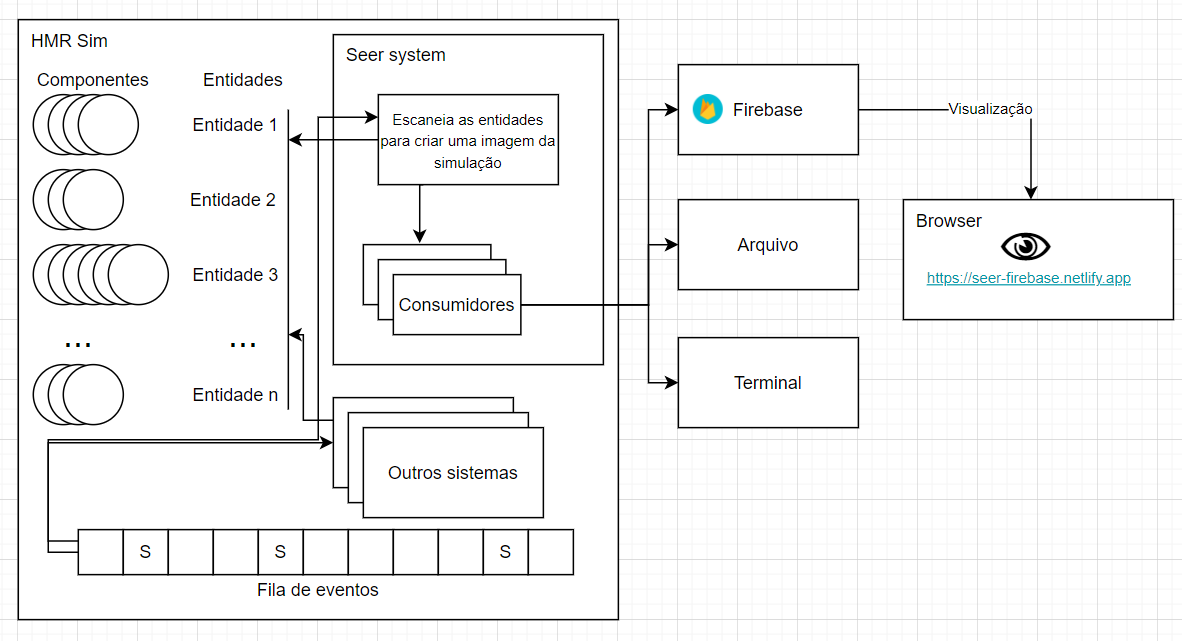
\includegraphics[width=\textwidth]{seer_architecture.png}
    \caption{Esquema da arquitetura do sistema Seer}
    \label{fig:seer_architecture}
\end{figure}

Seer é um sistema opcional como qualquer outro. A figura \ref{fig:seer_architecture} mostra um esquema da arquitetura desse sistema, feito para ser extensível. Ele utiliza os componentes \texttt{Position} e \texttt{Skeleton}, esse segundo sendo utilizado para guardar o estilo das entidades no XML do mapa. A cada evento do Seer (ilustrados na figura \ref{fig:seer_architecture} pelos espaços marcados com 'S' na fila de eventos) o sistema escaneias as entidades e cria uma mensagem que representa uma "fotografia" (e.g. \textit{snapshot}) da simulação naquele ponto. A frequência com que o Seer tira essas fotografias é especificado na inicialização do sistema. 

Criada a mensagem representando o estado da simulação em um ponto ela é colocada numa fila de mensagens. O gerenciador dos consumidores, que executa numa thread separada do simulador, remove as mensagens dessa fila e as passa para uma lista de consumidores. Esses consumidores são funções que vão processar as mensagens, e possivelmente enviá-las para outros locais de armazenamento, como mostrado na figura. Os consumidores são passados para o Seer no momento de sua inicialização, e podem ser criados para atender às necessidades particulares do usuário. 

Um consumidor de destaque, representado na figura pelo caminho que vai até o Firebase e está conectado ao browser é o consumidor do firebase. Esse consumidor utiliza o banco de dados em tempo real do firebase para enviar as mensagens ao firebase. Um programa auxiliar que faz a tradução das mensagens no firebase e reconstroi a simulação é disponibilizado no endereço \url{https://seer-firebase.netlify.app}. Ele tem suporte a múltiplas simulações, e também permite visualizar os logs da simulação (ver figura \ref{fig:dullens_big_contribution}). A visualização da simulação em si utiliza a mesma biblioteca \texttt{jGraph} que a construção do mapa, para manter o máximo de compatibilidade, e pode ser executada passo a passo ou em sequência como um vídeo. As mensagens ficam salvas no banco de dados do Firebase e podem ser vistas depois, permitindo analises posteriores à simulação sem a necessidade de re-executar a simulação toda, um processo que pode ser custoso e demorado. 

Outro sistema que exemplifica a possibilidade de extrair informações da simulação é o sistema \texttt{ClockSystem}, que registra o tempo gasto para simular 1 segundo da simulação e guarda essa informação em um arquivo externo.

\begin{figure}
    \centering
    \begin{subfigure}[b]{0.4\textwidth}
        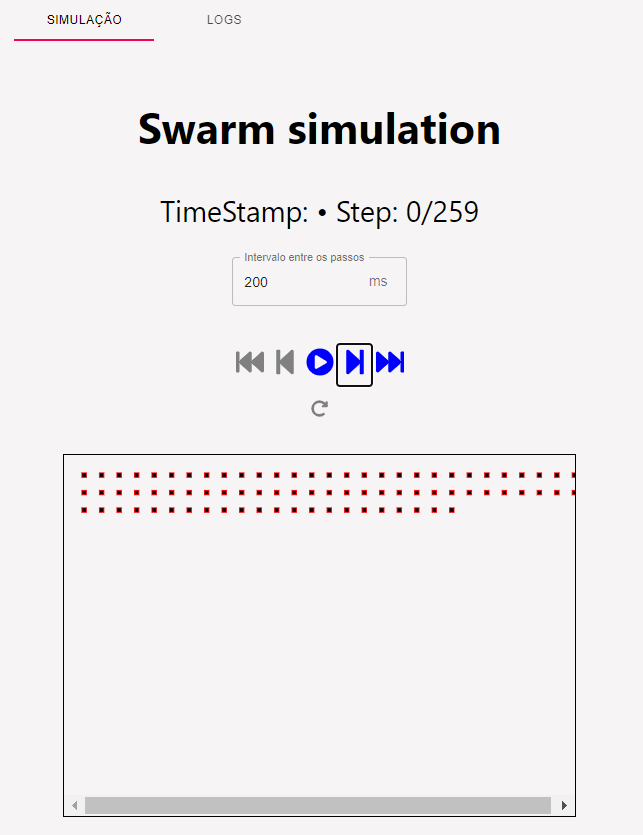
\includegraphics[width=\textwidth]{seer_simulation.png}
    \end{subfigure}
    \hfill
    \begin{subfigure}[b]{0.5\textwidth}
        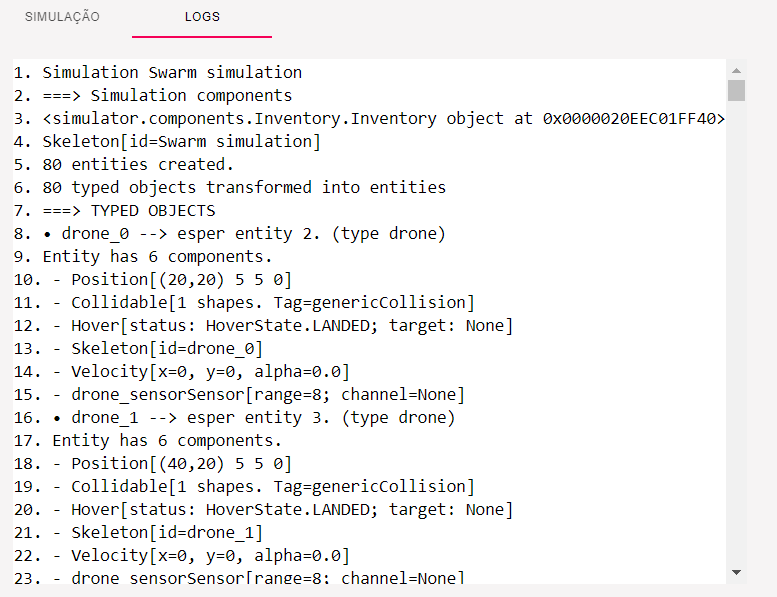
\includegraphics[width=\textwidth]{seer_logs.png}
    \end{subfigure}
    \caption{Visualizador do Seer disponível em \url{https://seer-firebase.netlify.app}}
    \label{fig:dullens_big_contribution}
\end{figure}

\section{Desempenho}
\label{sec:performance}

Um dos objetivos desse projeto é ter um simulador capaz de simular grandes times de robôs (50-200) de maneira eficiente. Para medir o desempenho do simulador nessas condições foi utilizada uma simulação de enxame de drones, aumentando a quantidade de drones de 20 até 200, e marcando quanto tempo demorou o tempo de processamento de 1 segundo da simulação ao longo da simulação. 

A simulação pode ser descrita da seguinte maneira: “Um controlador que conhece configuração para os drones tomarem. Temos uma quantidade grande de drones disponíveis. O controlador decide qual posição na configuração cada drone deve tomar e informa o drone qual sua posição. Cada drone deve tentar movimentar-se até a posição alvo sem bater nos outros drones. Ao chegar em sua posição, deve informar ao controlador e manter sua posição. Se ele bater em outro drone no caminho deve informar ao controlador. O controlador espera a resposta de todos os drones, ou um tempo máximo de 15s antes de encerrar a simulação".

Essa simulação foi construída programaticamente. A posição inicial e a posição final dos drones na simulação com 80 drones é mostrada na figura \ref{fig:drone_swarm}. Essa simulação pode ser vista pelo visualizador do Seer no usuário "simulator".

\begin{figure}
    \centering
    \begin{subfigure}[b]{0.4\textwidth}
        \centering
        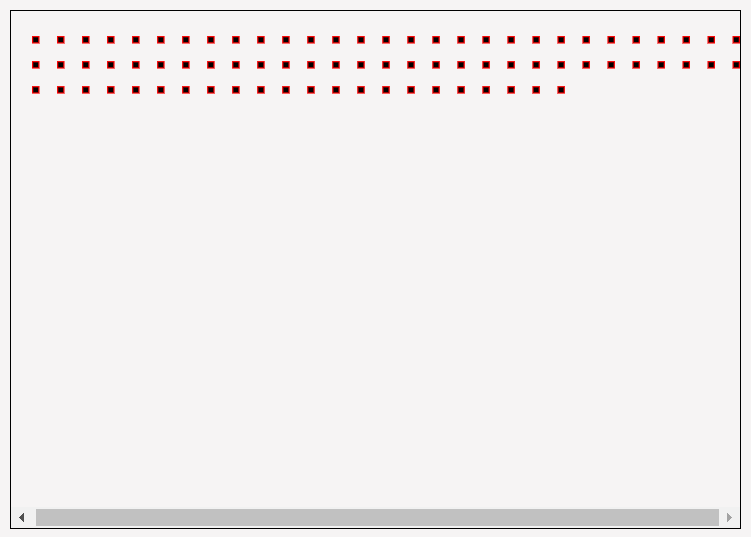
\includegraphics[width=\textwidth]{drone_swarm_init.png}
        \subcaption{Configuração inicial}
    \end{subfigure}
    \hfill
    \begin{subfigure}[b]{0.4\textwidth}
        \centering
        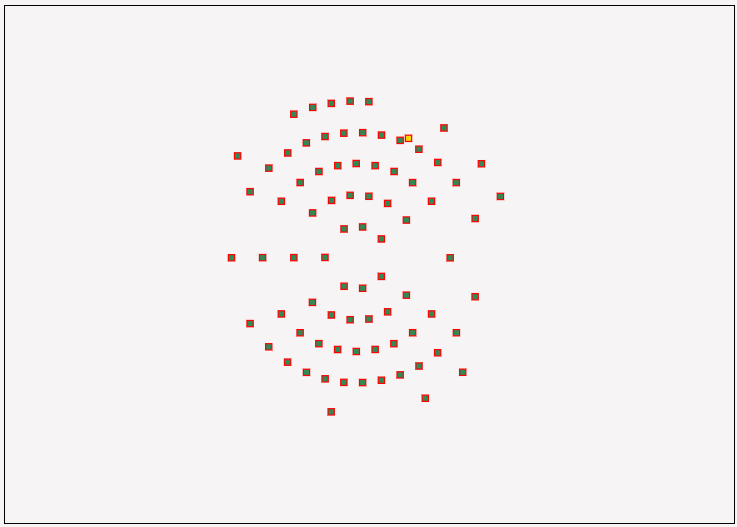
\includegraphics[width=\textwidth]{drone_swarm_end.png}
        \subcaption{Configuração final}
    \end{subfigure}
    \caption{Configurações inicial e final do enxame com 80 drones}
    \label{fig:drone_swarm}
\end{figure}

A tabela \ref{table:performance} mostra um resumo do desempenho do simulador com quantidades diferentes de drones. Tempo simulado é o tempo total da simulação, tempo mínimo e máximo são o menor e maior tempo do relógio necessário para computar 1s de simulação. Média é a média total em segundos do tempo do relógio para se computar 1s de simulação. A diferença no tempo necessário para computar um segundo de simulação está relacionado à posição dos drones ao longo da simulação. Nessa simulação, com 80 drones o tempo da simulação está aproximadamente sincronizado com o tempo do relógio.

\begin{table}
    \begin{tabular}{ccccccc}
        \toprule
        Nº de Drones &  Tempo Simulado &  Min. tempo 1s &  Max. tempo 1s &  Média \\
        \midrule
        20  &                8s &       0.0979s &       0.1778s &  0.1414s \\
        40  &               10s &       0.2700s &       0.3969s &  0.3458s \\
        60  &               20s &       0.4404s &       0.8829s &  0.6042s \\
        80  &               23s &       0.6978s &       1.3350s &  0.9698s \\
        100 &               22s &       0.9491s &       2.3663s &  1.4146s \\
        150 &               25s &       1.7435s &       3.0516s &  2.3176s \\
        200 &               32s &       3.1433s &       4.4711s &  3.7685s \\
        \bottomrule
    \end{tabular}
    \caption{Desempenho do simulador na simulação de enxame de drones por número de drones}
    \label{table:performance} 
\end{table}

A figura \ref{fig:time_process_across} mostra amédia de tempo de relógio necessário para computar 1s de simulação em função da quantidade de drones simulados. Fazendo a aproximação da função do gráfico com regressão quadrática obtemos a função $0.0001x^2+0.0087x-0.0641$, com média de erro relativo de 4.57\%. Usando regressão de expoente o resultado é $0.0018x^{1.4322}$, com erro relativo de 4.23\%. Isso indica que o aumento de entidades nessa simulação acarreta um aumento do tempo da simulação de forma polinomial, com um coeficiente próximo de 2.

A figura \ref{fig:drone_times} mostra como a média de tempo de relógio necessário para computar 1s de simulação muda ao longo da simulação, com números diferentes de drones. É possível observar que independente da natureza dos drones, existe uma tendência de aumento do tempo médio até um pico e depois uma queda até o final da simulação. Isso acontece devido à natureza da simulação. Inicialmente todos os drones estão a uma distância constante (veja figura \ref{fig:drone_swarm}), conforme o controlador assinala posições aos drones eles começam a se movimentar na direção do centro do mapa e ficam mais próximos uns dos outros (ver figura \ref{fig:time_peak}), causando um aumento no tempo de processamento (principalmente devido ao sistema de colisão). Conforme os drones chegam nas suas posições (ver figura \ref{fig:drone_swarm}) o número de entidades ativamente se movendo diminui, e com isso o tempo de processamento médio também. Isso indica que a natureza da simulação afeta diretamente o desempenho do simulador.

\begin{figure}[ht]
    \centering
    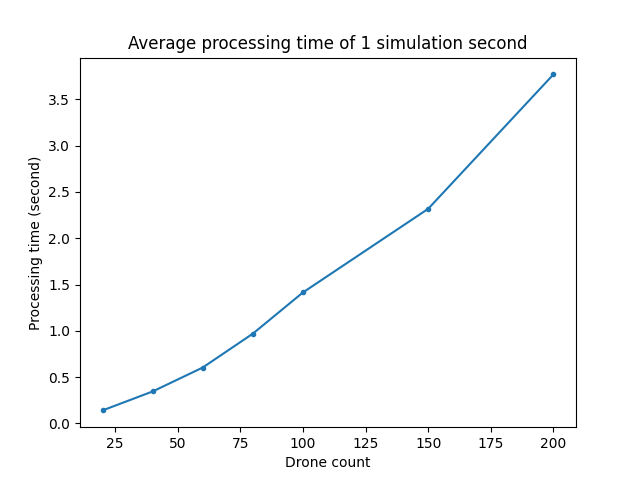
\includegraphics[width=\textwidth]{time_process_1s_across_simulations.png}
    \caption{Tempo para processar 1s de simulação por número de drones}
    \label{fig:time_process_across}
\end{figure}


\begin{figure}
    \centering
    \begin{subfigure}[b]{0.4\textwidth}
        \centering
        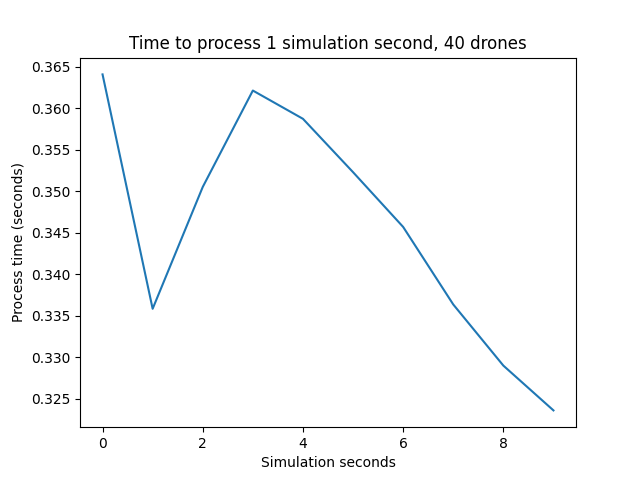
\includegraphics[width=\textwidth]{time_process_1s_simulation_40drones.png}
        \subcaption{40 drones}
    \end{subfigure}
    \hfill
    \begin{subfigure}[b]{0.4\textwidth}
        \centering
        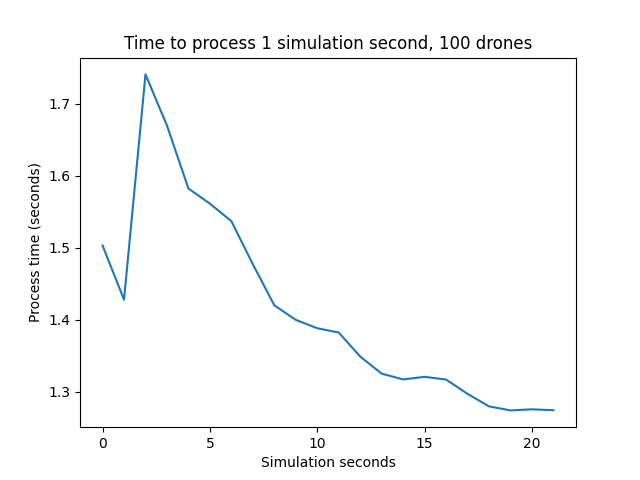
\includegraphics[width=\textwidth]{time_process_1s_simulation_100drones.png}
        \subcaption{100 drones}
    \end{subfigure}
    \begin{subfigure}[b]{0.5\textwidth}
        \centering
        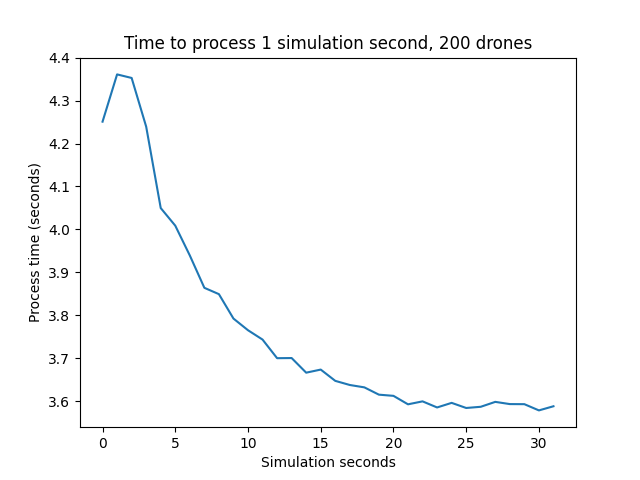
\includegraphics[width=\textwidth]{time_process_1s_simulation_200drones.png}
        \subcaption{200 drones}
    \end{subfigure}
    \caption{Tempo médio para computar 1s de simulação ao longo da simulação com 40, 100 e 200 drones}
    \label{fig:drone_times}
\end{figure}

\begin{figure}[ht]
    \centering
    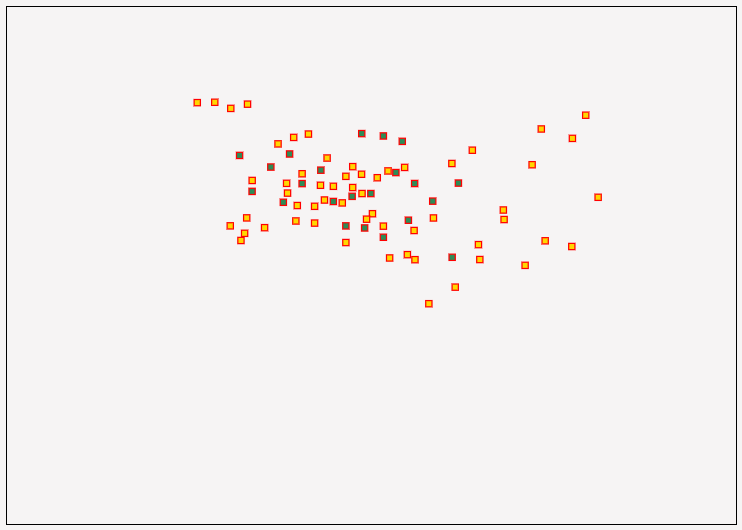
\includegraphics[width=.8\textwidth]{swarm_peak.png}
    \caption{Drones próximos uns dos outros ao longo da simulação. Pontos verdes são drones pairando em sua posição. Pontos amarelos são drones movendo-se para sua posição }
    \label{fig:time_peak}
\end{figure}